% Format teze zasnovan je na paketu memoir
% http://tug.ctan.org/macros/latex/contrib/memoir/memman.pdf ili
% http://texdoc.net/texmf-dist/doc/latex/memoir/memman.pdf
% 
% Prilikom zadavanja klase memoir, navedenim opcijama se podešava 
% veličina slova (12pt) i jednostrano štampanje (oneside).
% Ove parametre možete menjati samo ako pravite nezvanične verzije
% mastera za privatnu upotrebu (na primer, u b5 varijanti ima smisla 
% smanjiti 
\documentclass[12pt,oneside]{memoir} 

% Paket koji definiše sve specifičnosti master rada Matematičkog fakulteta
\usepackage[latinica]{matfmaster} 
\usepackage{xcolor}
\usepackage{listings}
% \documentclass{article}
\usepackage{cmsrb}
\usepackage[OT2,T1]{fontenc} %better to use T1, but OT1 will also work
% \usepackage[serbian]{babel}%
% Podrazumevano pismo je ćirilica.
%   Ako koristite pdflatex, a ne xetex, sav latinički tekst na srpskom jeziku
%   treba biti okružen sa \lat{...} ili \begin{latinica}...\end{latinica}.
%
% Opicija [latinica]:
%   ako želite da pišete latiniciom, dodajte opciju "latinica" tj.
%   prethodni paket uključite pomoću: \usepackage[latinica]{matfmaster}.
%   Ako koristite pdflatex, a ne xetex, sav ćirilički tekst treba biti
%   okružen sa \cir{...} ili \begin{cirilica}...\end{cirilica}.
%
% Opcija [biblatex]:
%   ako želite da koristite reference na više jezika i umesto paketa
%   bibtex da koristite BibLaTeX/Biber, dodajte opciju "biblatex" tj.
%   prethodni paket uključite pomoću: \usepackage[biblatex]{matfmaster}
%
% Opcija [b5paper]:
%   ako želite da napravite verziju teze u manjem (b5) formatu, navedite
%   opciju "b5paper", tj. prethodni paket uključite pomoću: 
%   \usepackage[b5paper]{matfmaster}. Tada ima smisla razmisliti o promeni
%   veličine slova (izmenom opcije 12pt na 11pt u \documentclass{memoir}).
%
% Naravno, opcije je moguće kombinovati.
% Npr. \usepackage[b5paper,biblatex]{matfmaster}

% Pomoćni paket koji generiše nasumičan tekst u kojem se javljaju sva slova
% azbuke (nema potrebe koristiti ovo u pravim disertacijama)
% \usepackage[latinica]{pangrami}

% Datoteka sa literaturom u BibTex tj. BibLaTeX/Biber formatu
\bib{MasterRadOgnjenPlavsic}

% Ime kandidata na srpskom jeziku (u odabranom pismu)
\autor{Ognjen Ž. Plavšić}
% Naslov teze na srpskom jeziku (u odabranom pismu)
\naslov{Alat za stati\v{c}ku analizu i predlaganje izmena u C++ kodu}
% Godina u kojoj je teza predana komisiji
\godina{2022}
% Ime i afilijacija mentora (u odabranom pismu)
\mentor{dr Milena \textsc{Vujošević Janičić}, vanredni profesor\\ Univerzitet u Beogradu, Matematički fakultet}
% Ime i afilijacija prvog člana komisije (u odabranom pismu)
\komisijaA{dr Filip \textsc{Marić}, vanredni profesor\\ Univerzitet u Beogradu, Matematički fakultet}
% Ime i afilijacija drugog člana komisije (u odabranom pismu)
\komisijaB{dr Jelena \textsc{Graovac}, docent\\ Univerzitet u Beogradu, Matematički fakultet}
% Ime i afilijacija trećeg člana komisije (opciono)
% \komisijaC{}
% Ime i afilijacija četvrtog člana komisije (opciono)
% \komisijaD{}
% Datum odbrane (odkomentarisati narednu liniju i upisati datum odbrane ako je poznat)
% \datumodbrane{}

% Apstrakt na srpskom jeziku (u odabranom pismu)
\apstr{%
% \pangrami
}
\usepackage{tcolorbox}
% Ključne reči na srpskom jeziku (u odabranom pismu)
\kljucnereci{računarstvo, autosar, clang, llvm, c++}

\begin{document}
% ==============================================================================
% Uvodni deo teze
\frontmatter
% ==============================================================================
% Naslovna strana
\naslovna
% Strana sa podacima o mentoru i članovima komisije
\komisija
% Strana sa posvetom (u odabranom pismu)
\posveta{Porodici}
% Strana sa podacima o disertaciji na srpskom jeziku
\apstrakt
% Sadržaj teze
\tableofcontents*

% ==============================================================================
% Glavni deo teze
\mainmatter
% ==============================================================================

% ------------------------------------------------------------------------------
\chapter{Uvod}
% ------------------------------------------------------------------------------
% \pangrami

% \section{Primeri korišćenja klasičnih \LaTeX{} elemenata}
% % Primeri citiranja
% Još jedan citat \cite{GuSh:243}.
% % Primeri navodnika
% Isprobavamo navodnike: "Rekao je da mu se javimo sutra".
% % Primer referisanja na tabelu (koja se javlja kasnije)
% U tabeli \ref{tbl:rezultati} koja sledi prikazani su rezultati eksperimenta.
% % Primer kraćeg ćiriličkog teksta
% {\cir Ово је пример ћириличког текста који се јавља у латиничком документу.}
% U ovoj rečenici se javlja jedna reč na {\cir ћирилици}.
% % Primer korišćenja fusnota
% Iza ove rečenice sledi fusnota.\footnote{Ovo je fusnota.}

% % Primer dužeg ćirličkog teksta
% \begin{cirilica}
%   Ово је мало дужи блок текста исписан ћириличким писмом у оквиру
%   латиничког документа. Фијуче ветар у шибљу, леди пасаже и куће иза
%   њих и гунђа у оџацима.
% \end{cirilica}

% % Primer korišćenja tabele
% \begin{table}
% \centering
% \caption{Rezultati}
% \label{tbl:rezultati}
% \begin{tabular}{c>{\centering}p{2cm}c}
% \toprule
% 1 & 2 & 3\\\midrule
% 4 & 5 & 6\\\cmidrule(rl){1-2}
% 7 & 8 & 8\\
% \bottomrule
% \end{tabular}
% \end{table}

% % Primer korišćenja slike
% \begin{figure}[!ht]
%   \centering
%   \label{fig:grafikon}
%   \includegraphics[width=0.5\textwidth]{graph.png}
%   \caption{Grafikon}
% \end{figure}


% % Primer jednostavnije matematičke formule
% Evo i jedan primer matematičke formule: $e^{i\pi} + 1 = 0$. 
% % Primer referisanja na sliku
% Na slici \ref{fig:grafikon} prikazan je jedan grafikon.

% % primer kompleksnije matematičke formule
% $$
% \int_a^b f(x)\ \mathrm{d}x \ =_{def}\ \lim_{\max{\Delta x_k \rightarrow 0}} \sum_{k=1}^n f(x_k^*)\Delta x_k
% $$

% % primer referisanja na poglavlja i strane poglavlja
% Više detalja biće dato u glavi \ref{chp:razrada} na strani \pageref{chp:razrada}.

% % primer liste
% Možemo praviti i nabrajanja:
% \begin{enumerate}
% \item Analiza 1
% \item Linearna algebra
% \item Analitička geometrija
% \item Osnovi programiranja
% \end{enumerate}

% \pangrami

% ------------------------------------------------------------------------------

\chapter{Programski jezik C++}
\label{chp:autosar}

\textbf{C++} je programski jezik op\v{s}te namene koji pru\v{z}a direktan i efikasan model hardvera u kombinaciji sa strukturama za definisanje lakih (eng. \textit{lightweight}) apstrakcija \cite{TheC++ProgrammingLanguage}. Kreirao ga je Danski softverski in\v{z}enjer Bjarne Stroustrup kao ekstenziju programskog jezika C. Osnovno pro\v{s}irenje u odnosu na programski jezik C jeste mogu\'{c}nost kreiranja korisni\v{c}ki definisanih tipova, odnosno klasa. C++ pripada grupi objektno orijentisanih jezika. 

\section{Dizajn programskog jezika C++}

Programski jezik C dizajniran je sa ciljem da programer mo\v{z}e sto jednostavnije zadavati akcije koje ma\v{s}ina treba da izvr\v{s}i.
Osnovna ideja iza dizajna programskog jezika C++ jeste da zadr\v{z}i dizajn jezika C ali ga i pro\v{s}iri tako da jezik, odnosno njegova sintaksa, bude bliska problemu koji re\v{s}ava. Tako implementiranim programskim jezikom se koncepti re\v{s}enja problema mogu izraziti direktno i koncizno.
U svrhu toga, C++ pru\v{z}a:
\begin{itemize}
  \item {Direktna mapiranja ugrađenih operacija i tipova na hardver kako bi obezbedio efikasno kori\v{s}\'{c}enje memorije i efikasne niske (eng. \textit{low-level}) operacije.}
  \item {Priu\v{s}tive (u smislu ra\v{c}unarskih resursa) i fleksibilne mehanizme apstrakcija za podr\v{s}ku korisni\v{c}ki definisanih tipova koji se mogu koristiti sa istom sintaksom, u istom obimu i sa istim performansama kao ugrađeni tipovi.}
\end{itemize}

Dizajn C++-a je fokusiran na tehnike programiranja koje se bave osnovnim pojmovima ra\v{c}unarstva kao \v{s}to su memorija, mutabilnost, apstrakcija, upravljanje ra\v{c}unarskim resursima, izra\v{z}avanje algoritama, rukovanje gre\v{s}kama i modularnost. Jezik je dizajniran sa ciljem da \v{s}to vi\v{s}e olak\v{s}a sistemsko programiranje, odnosno pisanje programa koji direktno koriste hardverske resurse i kod kojih su ovi resursi u velikoj meri ograni\v{c}eni \cite{TheC++ProgrammingLanguage}.


\section{Standard C++14}

Programski jezik C++ je standardizovan od strane ISO (\textit{International Standard Organization}) radne grupe poznate kao JTC1/SC22/WG21 \cite{ISOWebsite}. Do sada je objavljeno \v{s}est revizija C++ standarda i trenutno se radi na reviziji \textit{C++23}. 
\indent

Standard \textit{C++14} predstavlja pro\v{s}irenje standarda \textit{C++11} uglavnom manjim pobolj\v{s}anjima i ispravljanjem gre\v{s}aka iz standarda \textit{C++11} . Standard \textit{C++11} sa druge strane uveo je velike izmene u odnosu da prethodnu reviziju standarda, \textit{C++03}. 
Standardi \textit{C++11/14} uveli su ve\'{c}inu fundamentalnih koncepta onog \v{s}to se danas smatra modernim C++-om. Ovde pre svega spadaju desne reference, "move" semantika i savr\v{s}eno prosleđivanje, pametni pokaziva\v{c}i, lambda funkcije, dedukcija tipova ali i mnogi drugi koncepti.


\chapter{Standard kodiranja Autosar C++14}
\label{chp:autosar}


\textit{AUTomotive Open System ARchitecture (AUTOSAR)} je međunarodna organizacija proizvođača vozila, dobavljača, pružaoca usluga i kompanija iz automobilske industrije i industrija elektronike, poluprovodnika i softvera \cite{AutosarWebsite}. 
Cilj Autosara je da stvori i uspostavi otvorenu i standardizovanu softversku arhitekturu za automobilske elektronske upravljačke jedinice (\textit{eng. Electronic Control Units (ЕCU)}.
Radi ostvarenja pomenutih ciljeva AUTOSAR definiše, između ostalog, pravila kodiranja u programskom jeziku C++14 za sigurnosno kriti\v{c}ne sisteme. Glavni sektor primene standarda kodiranja AUTOSAR C++14 je automobilska industrija, međutim ovaj standard može biti primenjen
i na druge aplikacije za uređaje sa ugrađenim računarom (\textit{eng. embedded systems}). Ovaj standard predstavlja nadogradnju MISRA C++:2008 standarda \cite{AutosarGuidelines}.

\section{Klasifikacija pravila}
Standard AUTOSAR C++14 definiše 342 pravila od kojih je:
\begin{itemize}
  \item {154 prisvojeno bez modifikacija iz MISRA C++:2008 standarda.}
  \item {131 prisvojeno iz drugih C++ standarda}
  \item {57 pravila je zasnovano na istraživanju, literaturi ili iz drugih resursa.}
\end{itemize}
Pravila su klasifikovana po nivou obaveze, mogućnosti ispitivanja saglasnosti koda sa pravilom korišćenjem algoritama
statičke analize i cilju korišćenja:

\begin{itemize}
  \item{
Klasifikacija po nivou obaveze deli pravila na obavezna i preporučena.
Obavezna pravila predstavljaju neophodne zahteve koje C++ k\^{o}d mora ispuniti kako bi bio u saglasnosti sa standardom. U slučaju kada ovo nije moguće,
formalna odstupanja moraju biti prijavljena.
Preporučena pravila predstavljaju zahteve koje C++ k\^{o}d treba da ispuni kad god je to mogu\'{c}e. Međutim, ovi zahtevi nisu obavezni. Pravila
sa ovim nivoom obaveze ne treba smatrati savetom ili sugestijom koja može biti ignorisana ve\'{c} ih treba pratiti uvek kada je to prakti\v{c}no izvodljivo. Za ova pravila ne moraju biti prijavljena formalna odstupanja.}

  \item{
Klasifikacija po primenjivosti statičke analize deli pravila na: 
\begin{enumerate}
  \item{automatizovana}
  \item{delimično automatizovana}
  \item{neautomatizovana}
\end{enumerate}
Automatizovana su ona pravila kod kojih se ispitivanje saglasnosti koda može u potpunosti automatizovati algoritmima statičke analize.
Kod delimično automatizovanih pravila se ispitivanje saglasnosti koda može samo delimilčno automatizovati, na primer, korišćenjem neke heuristike ili pokrivanjem određenog broja slučajeva upotrebe i služi kao dopuna pregleda koda.
Za neautomatizovana pravila statička analiza ne pruža razumnu podršku. Za ispitivanje saglasnosti koda sa neautomatizovanim pravilima koriste se druga sredstva, kao što je recimo pregled koda.

\indent
Većina pravila iz standarda Autosar C++14 spadaju u automatizovana pravila. Alati za statičku analizu koda koji tvrde da podržavaju standard Autosar C++14 moraju u potpunosti obezbediti podršku za sva automatizovana pravila i delimičnu podršku, u meri u kojoj je to moguće, za pravila koja se ne mogu u potpunosti ispitati algoritmima statičke analize \cite{AutosarGuidelines}.

\indent
Primenjivost statičke analize na proveru saglasnosti koda sa određenim pravilom u velikoj meri zasniva se na teorijskoj klasifikaciji problema
na odlučive i neodlučive probleme. Ukoliko se pravilo zasniva na neodlučivom problemu možemo sa sigurnošću reći da alati za statičku analizu nisu u mogućnosti da u potpunosti ispitaju saglasnost koda sa ovim pravilom. Pravilo će biti klasifikovano kao parcijalno automatizovano ili neautomatizovano ukoliko detektovanje kršenja pravila obuhvata određivanje vrednosti koju promenljiva sadrži u fazi izvr\v{s}avanja ili da li program doseže određeni deo programa.

Primer parcijalno automatizovanog pravila je: 

\begin{center}
% [title=My heading line]

\begin{tcolorbox}
 M5-8-1 (obvezno, implementaciono, parcijalno automatizovano) \\
Desni operand šift operacije treba biti manji za broj između nula i jedan
od bitske širine tipa levog operanda.

\end{tcolorbox}
\end{center}

  % \textit{Pravilo M5-8-1 (obvezno, implementaciono, parcijalno automatizovano)
  %         Desni operand šift operacije treba biti manji između nula i jedan od bitske širine tipa levog operanda.} \\ \\
  Pravilo nije moguće u potpunosti automatizovati jer je očigledno potrebno poznavati vrednost desnog operanda, što u opštem slučaju nije
  moguće precizno zaključiti. Primer ovakvog koda prikazan je na listingu 2.1. 
\begin{english}
\lstset{%
language=C,
frame=single,
numbers=left,
numberstyle=\footnotesize,
tabsize=2,
keepspaces=true,
columns=fullflexible,
basicstyle=\ttfamily\scriptsize,
keywordstyle=\color{blue}
}



\begin{lstlisting}[caption={K\^{o}d koji ilustruje nemogućnost primene statičke analize},label={lst:label},language=C++, captionpos=b]
#include <iostream>
#include <cstdint>
#include <cstdlib>

int main(){
int8_t u8a = rand() % 100;
u8a = (uint8_t) ( u8a << rand() % 10);
}
\end{lstlisting}
\end{english}
Međitim, ukoliko je desni operand konstanta ili promenljiva konstantnog izraza (klju\v{c}na re\v{c} \textit{constexpr}), vrlo je verovatno da će alat za statičku analizu biti u stanju
  da zaključi vrednost ove promenljive (s obzirom da su ove vrednosti poznate tokom kompilacije), a samim tim i ispitati saglasnost koda sa ovim pravilom.
  Primer ovakvog koda prikazan je na Listingu 2.2.
\begin{english}
\lstset{%
language=C,
frame=single,
numbers=left,
numberstyle=\footnotesize,
tabsize=2,
keepspaces=true,
columns=fullflexible,
basicstyle=\ttfamily\scriptsize,
keywordstyle=\color{blue}
}



\begin{lstlisting}[caption={K\^{o}d čija se ispravnost jednostavno može utvrditi statičkom analizom},label={lst:label},language=C++, captionpos=b]
#include <iostream>
#include <cstdint>
#include <cstdlib>

int main(){
int8_t u8a = rand() % 100;
u8a = (uint8_t) ( u8a << 7);
}
\end{lstlisting}
\end{english}

  Napredniji alati za statičku analizu koji podržavaju simboličko izvršavanje programa (npr. Clang Static Analyzer \cite{CSAWebsite}) mogu pokriti i znatno kompleksnije 
  slučajeve od slučaja prikazanog u Listingu 2.2.
  \\
  \indent 
  Ukoliko su pravila koja se odnose na implementaciju C++ projekta, odnosno na C++ konstrukte i semantiku programa, dovoljno kompleksna, može se desiti da u potpunosti nije moguće koristiti alate za statičku analizu. Ovo uglavnom znači da je broj slučajeva upotrebe koji algoritmi iz statičkih alata mogu pokriti, zanemarljiv. Međutim, određeni broj pravila koja su klasifikovana kao neautomatizovana odnose se na aspekte koda koji zavise od samog projekta
  u okviru kog je k\^{o}d napisan, stoga je nemoguće koristiti algoritme statičke analize.
  Primer ovakvog pravila je:

\begin{center}
\begin{tcolorbox}
Pravilo A1-4-2 (obvezno, implementaciono, neautomatizovano) \\
Kod treba da poštuje zadate granice metrika koda.
\end{tcolorbox}
\end{center}

  %  \\ \\
  % \textit{Pravilo A1-4-2 (obvezno, implementaciono, neautomatizovano)
  %         Sav k\^{o}d treba poštovati definisane granice metrika koda.} \\

  Kako bi se odredilo da li je k\^{o}d napisan u skladu sa ovim pravilom potrebno je poznavati koje metrike koda se koriste u okviru projekta i
  granice definisane za te metrike. S obzirom da je ovo specifično za sam projekat, mogu se koristiti interni alati za statičku analizu koda u kombinaciji
  sa manuelnim pregledom koda. 
}
  \item{
Klasifikacija pravila prema cilju primene (slučaju upotrebe) deli pravila na:

\begin{enumerate}
  \item{implementaciona}
  \item{verifikaciona}
  \item{pravila za alate}
  \item{infrastrukturna}
\end{enumerate}

Implementaciona pravila se odnose na implementaciju projekta odnosno na k\^{o}d, arhitekturu i dizajn.
Primer implementacionog pravila:

\begin{center}
\begin{tcolorbox}
Pravilo A2-9-1 (obvezno, implementaciono, automatizovano) \\
Ime heder fajla mora biti identično imenu tipa deklarisanog u njemu ukoliko deklariše tip.
\end{tcolorbox}
\end{center}


Verifikaciona pravila odnose se na proces verifikacije koji uključuje pregled koda, analizu i testiranje.
Primer verifikacionog pravila:

\begin{center}
\begin{tcolorbox}
Pravilo A15-0-6 (obvezno, verifikaciono, neautomatizovano) \\
Analiza treba biti izvršena kako bi se detektovalo loše rukovanje izuzecima. Treba analizirati slede\'ce slučajeve lošeg rukovanja izuzecima:
(a) Najgore vreme izvršavanja ne postoji ili se ne može utvrditi, \\
(b) Stek nije korektno raspakovan, \\
(c) Izuzetak nije bačen, drugačiji izuzetak je bačen, aktivirana je pogre\v{s}na "catch" naredba, \\
(d) Memorija nije dostupna tokom rukovanja izuzecima.
\end{tcolorbox}
\end{center}

Pravila za alate odnose se na softverske alate kao što su pretprocesor, kompajler, linker i biblioteke kompajlera.
Infrastrukturna pravila odnose se na operativni sistem i hardver \cite{AutosarGuidelines}.
Primer pravila za alate koje je ujedno i infrastrukturno pravilo:

\begin{center}
\begin{tcolorbox}
Pravilo A0-4-1 (obvezno, pravilo za infrastrukturu/alate, neautomatizovano) \\
Implementacija brojeva u pokretnom zarezu treba da bude u skladu sa standardom IEEE 754.
\end{tcolorbox}
\end{center}

}
\end{itemize}

\section{Opis implementiranih pravila}

Pored formalne klasifikacije opisane u prethodnom poglavlju, pravila u okviru samog dokumenta standarda AUTOSAR C++14  kodiranja struktuirana su po poglavljima.
Struktura poglavlja ovog dokumenta slična je strukturi iz samog C++ standarda ISO/IEC 14882:2014. Svako poglavlje odgovara jednoj komponenti (svojstvu) C++14 jezika, to jest, sadrži pravila koja se odnose na tu komponentu.
\\
\indent
Pravila razmatrana u ovom radu predstavljaju podskup pravila koja se odnose na deklaracije. Razlog za ovo je dvojak. Deklaracije predstavljaju jedan
od osnovnih i najvažnijih koncepta u C++-u i programiranju generalno. U C++-u deklaracije čine samu srž ekspresivne moći jezika i u direktnoj su vezi
sa naprednijim konceptima jezika i računarastva, kao što je, na primer, šablonsko metaprogramiranje (\textit{eng. template metaprogramming}).
Sa druge strane jednostavnost sintakse deklaracija u C++-u čini pogodno tlo za korišćenje kompajlerskih tehnika i struktura u okviru Clang kompajlera kojim se mogu analizirati konstrukti jezika koji nisu u skladu sa pravilima i predlagati prikladne alternative.
\\
\indent
Sva implementirana pravila u okviru projekta spadaju, prema klasifikaciji iz prethodnog poglavlja, u sledeće kategorije:
\begin{enumerate}
  \item{Obavezna, prema klasifikaciji po obavezi.}
  \item{Automatizovana, prema klasifikaciji po primenjivosti statičke analize.}
  \item{Implementaciona, prema klasifikaciji po cilju primene.}
\end{enumerate}

Razmatrana pravila nisu nužno implementirana u potpunosti u okviru Autofix alata, iako činjenica da pravila spadaju u kategorije obaveznih i automatizovanih
implicira da je to teorijski moguće uraditi. Pravila koje Autofix podržava birana su tako da se ograničenja koja potiču iz same prirode projekta minimalno manifestuju. Ograničenja potiču od primarnih tehnologija i biblioteka kojima je alat implementiran ali i činjenice da se alat zasniva na predlogu izmena koda. 
Clang Statički analizator (\textit{eng. Clang Static Analyzer} \cite{CSAWebsite}) nije korišćen u okviru ovog alata, tako da su pravila izabrana tako da što manji broj slučajeva upotrebe zahteva simboličko izvršavanje programa. Drugo ograničenje potiče iz činjenice da u nekim slučajevima nije moguće ili je znatno komplikovanije kreirati predlog ispravke koda (\textit{eng. fixit hint}). Pravila razmatrana u okviru ovog rada birana su tako da se većina konstrukta koji nisu u saglasnosti sa pravilom mogu detektovati analizom Clang-ovog AST-a i da se za njih mogu kreirati razumne alternative koje su u skladu sa standardom Autosar C++14.
Primeri pravila koje podržava Autofix alat:

\begin{center}
\begin{tcolorbox}
Pravilo A7-1-8 (obvezno, implementaciono, automatizovano) \\
U deklaracijama specifikatori koji nisu vezani za tipove treba da stoje
ispred tipskih specifikatora.
\end{tcolorbox}
\end{center}

\begin{center}
\begin{tcolorbox}
Pravilo A8-5-3 (obvezno, implementaciono, automatizovano) \\
Varijabla tipa \textbf{auto} ne sme biti inicijalizovana kori\v{s}\'{c}enjem
inicijalizacijom viti\v{c}astih zagrada tipa \{\} ili =\{\}.
\end{tcolorbox}
\end{center}

% % primer korišćenja slike
% \begin{figure}[!ht]
%   \centering
%   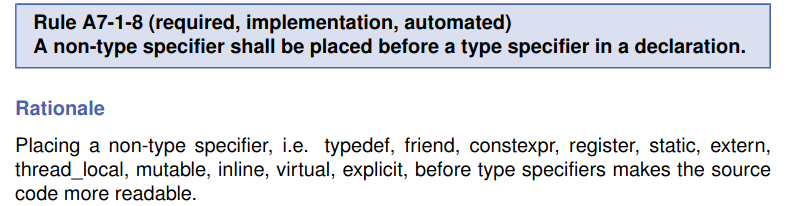
\includegraphics[width=0.5\textwidth]{PraviloA718.png}
%   \caption{Pravilo A7-1-8}
%   \label{fig:grafikon}
% \end{figure}

% \begin{figure}[!ht]
%   \centering
%   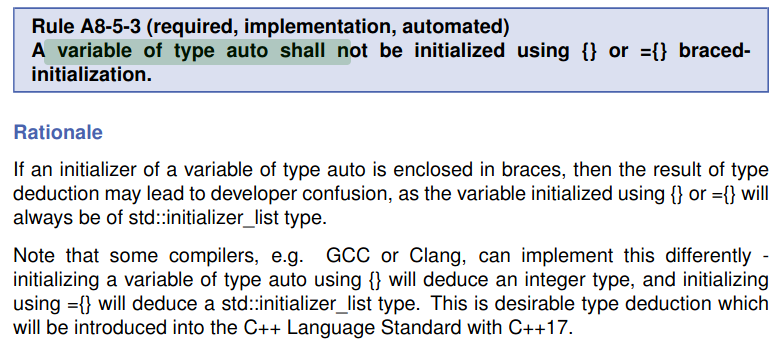
\includegraphics[width=0.5\textwidth]{PraviloA853.png}
%   \caption{Pravilo A8-5-3}
%   \label{fig:grafikon}
% \end{figure}

\chapter{LLVM (nije spremno za reivew)}
\label{chp:llvm}

LLVM projekat predstavlja kolekciju modularnih i ponovo iskoristivih kompajlerskih tehnologija i alata.
Započet je 2000. godine kao instražički projekat Krisa Latnera (\textit{eng. Chris Lattner}) i Vikrama Advea (\textit{eng. Vikram Adve}) na Univerzitetu Ilinois.

LLVM podržava kompilaciju različitih programskih programiskih jezika na mnoštvo različitih arhitektura hardvera. Jednostavnost dodavanja podrške kompilacije programskog jezika za hardversku arhitekturu omogućeno je fleksibilnim dizajnom kod kog je infrastruktura kompajlera ugrubo podeljena na 3 dela. Izvorni k\^{o}d podržanih jezika prevodi se u LLVM međukod bibliotekama koji predstavljaju prednji deo kompajlera (\textit{eng. frontend}). Zatim se nad međukodom vrši niz optimizacija koje su nezavisne od izvornog koda ali i ciljne arhitekture. Biblioteke koje implementiraju pomenute optimizacije čine srednji deo (\textit{eng. middleend}) infrastrukture LLVM-a. Poslednji deo dizajna čini zadnji deo (\textit{eng. backend}) kompajlera prilikom kog se generiše izvršni k\^{o}d za ciljnu arhitekturu od LLVM međukoda.

% \usepackage{float}
\begin{figure}[!h]
\begin{center}
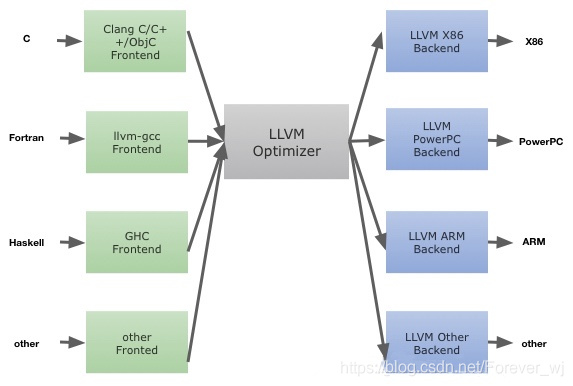
\includegraphics[scale=0.4]{llvmDesign.jpg}
\end{center}
\caption{Dizajn kompajlerske infrastrukture LLVM}
\label{fig:exploded}
\end{figure}

\section{Clang}

Clang projekat predstavlja prednji deo (\textit{eng. frontend}) LLVM kompajlerske infrastrukture za C familiju jezika (C, C++, Objective C/C++, OpenCL ...).
Pored optimizacija i efikasnog generisanja LLVM međukoda karakterističan je po ekspresivnosti dijagnostike odnosno kvalitetu poruka upozorenja i grešaka prijavljenih za izvorni kod. Dizajn Clang-a se sastoji od mnoštva biblioteka od kojih su najznačajnije za dizajn sledeće:

\begin{enumerate}
  \item{\textbf{Lekser i Predprocesor} \\
       Implementira leksičku analizu i predprocesiranje izvornog koda.
       Pruža mogućnost uključivanja datoteka zaglavlja, proširenja makroa, uslovne kompilacije i kontrole linija. 
       Kreira niz tokena od sintakse izvornog koda.}
  \item{\textbf{Parser} \\
        Kreira sintaksne strukture C++-a od niza tokena dobijenih leksičkom analizom.
        Clang-ov parser implementiran je kao parser rekurzivnog spuštanja, odnosno analizira izvorni kod od vrha ka dnu nizom rekurzivnih funkcija.}
  \item{\textbf{AST biblioteka} \\
        Ova biblioteka implementira algoritme i strukture podataka koje parser koristi za izgradnju AST-a. Specifična je po strukturi čvorova koji podsećaju na izvorni C++ kod što je čini pogodnim za kreiranje alata za refaktorisanje koda i statičku analizu.}
  \item{\textbf{Sema} \\
        Vrši semantičku analizu programa tokom parsiranja i od semantički validnih konstrukta kreira AST. Usko je povezana sa parserom i AST bibliotekom.}
  \item{\textbf{Biblioteka za generisanje koda (eng. CodeGen Library)} \\
        Dobija AST kao ulaz i od njega generiše LLVM međukod.}

\end{enumerate}

\begin{figure}[!ht]
  \centering
  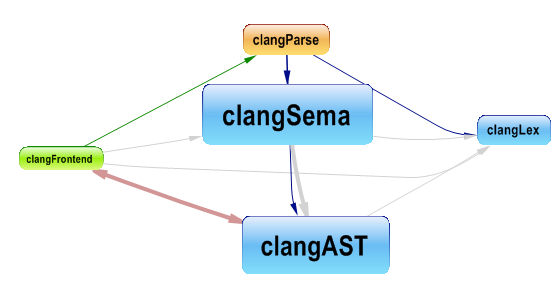
\includegraphics[width=0.6\textwidth]{ClangBiblioteke.png}
  \caption{Odnos osnovnih biblioteka Clang-a}
  \label{fig:grafikon}
\end{figure}

\section{AST biblioteka}

U računarstvu, \textbf{apstraktno sintaksno stablo} (eng. abstract syntax tree), ili samo \textbf{sintaksno stablo}, je drvoidna reprezentacija apstraktne sintaktičke strukture izvornog koda napisanog u programskom jeziku. Svaki čvor stabla predstavlja konstrukt koji se pojavljuje u izvornom kodu.
Sintaksa je apstraktna u smislu da ne predstavlja svaki detalj koji se pojavljuje u stvarnoj sintaksi, već samo strukturne ili detalje vezane za sadržaj.

Ekspresivnost Clang-ove dijagnostike i jednostavnost kreiranja mo\'{c}nih alata za stati\v{c}ku analizu u velikoj meri oslanja se na dizajn Clang-ove AST biblioteke. Struktura AST-a mo\v{z}e  se jednostavno ispisati na standardni izlaz Clang-ovom -ast-dump opcijom. Komanda na listingu 3.1 ispisuje na standardni izlaz AST za kod iz fajla hello.cpp prikazanog na listingu 3.2. Slika 3.1 predstavlja AST ispis dobijen komandom iz listinga 3.1.
\\
\lstset{%
language=C,
frame=single,
numbers=left,
numberstyle=\footnotesize,
tabsize=2,
keepspaces=true,
columns=fullflexible,
basicstyle=\ttfamily\scriptsize,
keywordstyle=\color{blue}
}

\begin{lstlisting}[caption={Komanda za ispisivanje Clang-ovog AST-a},label={lst:label},language=bash, captionpos=b]
$ clang -Xclang -ast-dump hello.c
\end{lstlisting}

\begin{lstlisting}[caption={Kod \v{c}iji je AST prikazan na slici 4.1},label={lst:label},language=C++, captionpos=b]
int main(){
  int a = 4;
  int b = 5;
  int result = a * b + 8;
}
\end{lstlisting}

% primer korišćenja slike
\begin{figure}[!ht]
  \centering
  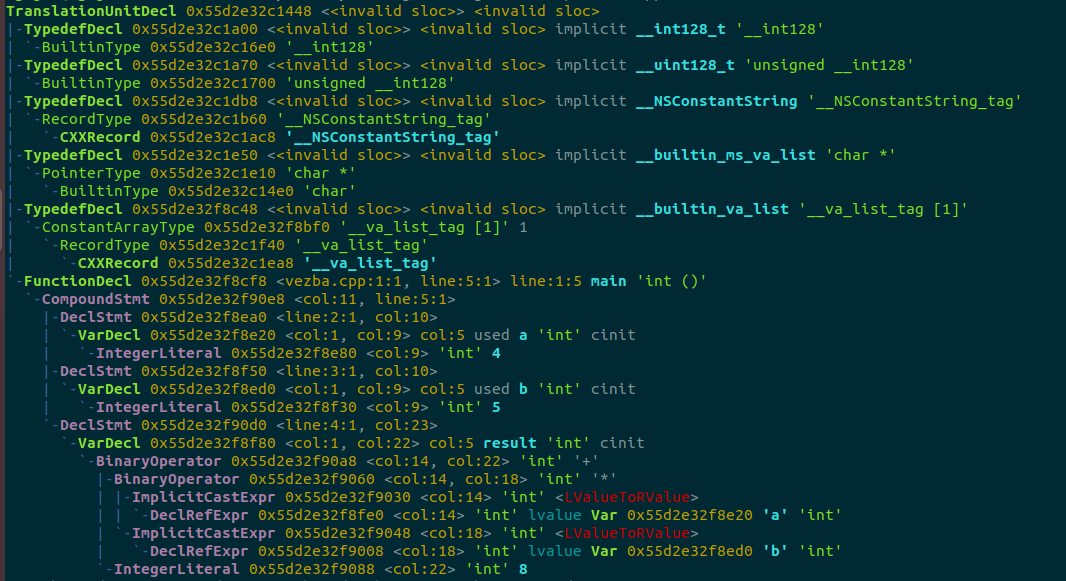
\includegraphics[width=0.7\textwidth]{ASTImage.png}
  \caption{Primer AST-a}
  \label{fig:grafikon}
\end{figure}

\v{C}vorovi od kojih je izgrađen AST predstavljaju apstrakciju sintaksnih struktura iz samog jezka.
Svi \v{c}vorovi Clang-ovog AST-a nasleđuju jednu od tri osnovne (bazne) klase:
\begin{itemize}
  \item \textit{Decl}
  \item \textit{Stmt}
  \item \textit{Type}
\end{itemize}
Ove klase redom opisuju deklaracije, naredbe i tipove iz C familije jezika.
Na primer IfStmt klasa opisuje 'if' naredbe jezika i direktno nasleđuje Stmt klasu. Sa druge strane FunctionDecl i VarDecl klase koje se koriste za opisivanje
deklaracija i definicija funkcija i varijabli (promenljivih) ne nasleđuju dikertno klasu Decl ve\'{c} nasleđuju vi\v{s}e njenih podklasa.

\begin{itemize}
  \item \textit{\textbf{Klasa Type}} \\ Tipovi igraju va\v{z}nu ulogu u ekspresivnosti Clang-ove dijagnostike. Dizajn ove klase klju\v{c}an je za preciznost emitovanih poruka upozorenja i gre\v{s}aka u kodu. Na primer, upozorenja vezana za kod koji koristi tip std::string, ispisa\'{c}e ba\v{s} taj tip u svojim porukama umesto tipa koji $std::string$ predefini\v{s}e, a to je $std::basic\_string<char, std:.. >$ . Iza ove funkcionalnosti stoji ideja kanonskih tipova.
  \\
  \indent
  Svaka instanca klase Type sadr\v{z}i pokaziva\v{c} na svoj kanonski tip. Za jednostavne tipove koji nisu definisani kori\'{c}enjem $typedef$ naredbe pokaziva\v{c} na kanonski tip \'{c}e zapravo pokazivati na sebe. Za tipove \v{c}ija struktura uklju\v{c}uje $typedef$ naredbu kanonski pokaziva\v{c} pokaziva\'{c}e na strukturno ekvivalentan tip bez $typedef$ naredbi.
  Na primer, kanonski tip tipa $int *$ sa listinga 3.3 bi\'{c}e sam taj tip, dok \'{c}e kanonski tip za \texttt{foo *} biti \texttt{int *}.
\begin{lstlisting}[caption={Demonstracija kanonskih tipova},label={lst:label},language=C++, captionpos=b]
  int *a;
  typedef int foo;
  foo *b;
\end{lstlisting}
  Ovakvim dizajnom omogu\'{c}no je semanti\v{c}kim proverama da donose zaklju\v{c}ke direktno o pravom tipu ignori\v{s}u\'{c}i \texttt{typedef} naredbe kao i efikasno poređenje strukturne identi\v{c}nosti tipova.
  \def\code#1{\texttt{#1}}
  \\
  \indent
  Klasa Type ne sadr\v{z}i informacije o kvalifikatorima tipova kao \v{s}to su \code{const}, \code{volatile}, \code{restrict} itd... Ove informacije enkapsulirane su u klasi \code{QualType} koja su\v{s}tinski predstavlja par pokaziva\v{c}a na tip (objekat klase \code{Type}) i bitova koji predstavljaju
  kvalifikatore. \v{C}uvanje kvalifikatora u vidu bitova omogu\'{c}uje veoma efikasno dohvatanje, dodavanje i brisanje kvalifikatora za tip. Postojanje ove klase smanjuje upotrebu hip memorije time \v{s}to se ne moraju kreirati duplikati tipova sa razli\v{c}itim kvalifikatorima. Na hipu se alocira jedan tip, a zatim 
  svi kvalifikovani tipovi pokazuju na alocirani tip na hipu sa dodatim kvalifikatorima.
\end{itemize}

\section{Tehnike stati\v{c}ke analize}

Kompajlerska infrastruktura LLVM pru\v{z}a podr\v{s}ku za jednostavno kreiranje kvalitetnih alata za stati\v{c}ku analizu izvornog koda. Ovi alati
baziraju se na kori\v{s}\'{c}enju interfejsa ka Clang-ovom AST-u ili kori\v{s}\'{c}enjem Clang-ovog stati\v{c}kog anlizatora (eng. \textit{Clang Static Analyzer}) za potrebe simboli\v{c}kog izvr\v{s}avanja programa. Alati za stati\v{c}ku analizu mogu koristiti kombinaciju tehnika obilaska AST-a i simboli\v{c}kog izvr\v{s}avanja programa u zavisnosti od kompleksnosti analize koja je potrebna. Biblioteke za obilazak AST-a su jeftinije za kori\v{s}\'{c}enje  po pitanju ra\v{c}unarskih resursa ali su ograni\v{c}ene informacijama dostupnim tokom kompilacije programa. Alati koji se implementiraju kao deo sistema za prevodjenje programa omogu\'{c}avaju dodatnu optimizaciju procesa pronala\v{z}enja nepravilnih konstrukta direktnim proverama tokom kompilacije. Ovo se mo\v{z}e posti\'{c}i nadogradnjom osnovnih delova kompajlera kao \v{s}to su Lexer, Parser ili Sema. \\Osnovne biblioteke za obilazak AST-a u okviru kompajlera Clang su AST posetioci (eng. \textit{ASTVisitors}) i  AST upariva\v{c}i (eng. \textit{ASTMatchers}).

% \usepackage{listings}
\definecolor{mygreen}{rgb}{0,0.6,0}
\definecolor{mygray}{rgb}{0.5,0.5,0.5}
\definecolor{mymauve}{rgb}{0.58,0,0.82}

\lstset{ 
  backgroundcolor=\color{white},   % choose the background color; you must add \usepackage{color} or \usepackage{xcolor}; should come as last argument
  basicstyle=\scriptsize\ttfamily,        % the size of the fonts that are used for the code
  breakatwhitespace=false,         % sets if automatic breaks should only happen at whitespace
  breaklines=true,                 % sets automatic line breaking
  captionpos=b,                    % sets the caption-position to bottom
  commentstyle=\color{mygreen},    % comment style
  deletekeywords={...},            % if you want to delete keywords from the given language
  escapeinside={\%*}{*)},          % if you want to add LaTeX within your code
  extendedchars=true,              % lets you use non-ASCII characters; for 8-bits encodings only, does not work with UTF-8
  firstnumber=1,                % start line enumeration with line 1000
  frame=single,                    % adds a frame around the code
  keepspaces=true,                 % keeps spaces in text, useful for keeping indentation of code (possibly needs columns=flexible)
  keywordstyle=\color{blue},       % keyword style
  language=Python,                 % the language of the code
  morekeywords={*,...},            % if you want to add more keywords to the set
  numbers=left,                    % where to put the line-numbers; possible values are (none, left, right)
  numbersep=5pt,                   % how far the line-numbers are from the code
  numberstyle=\tiny\color{mygray}, % the style that is used for the line-numbers
  rulecolor=\color{black},         % if not set, the frame-color may be changed on line-breaks within not-black text (e.g. comments (green here))
  showspaces=false,                % show spaces everywhere adding particular underscores; it overrides 'showstringspaces'
  showstringspaces=false,          % underline spaces within strings only
  showtabs=false,                  % show tabs within strings adding particular underscores
  stepnumber=1,                    % the step between two line-numbers. If it's 1, each line will be numbered
  stringstyle=\color{mymauve},     % string literal style
  tabsize=2,                     % sets default tabsize to 2 spaces
  title=\lstname,                   % show the filename of files included with \lstinputlisting; also try caption instead of title
  float=H
}

\newtheorem{primer}{Primer}[section]

\section{AST posetioci}
AST posetioci implementiraju mehanizam obilaska Clang-ovog AST stabla, odnosno pru\v{z}aju interfejs
za pose\'{c}ivanje svakog \v{c}vora u AST stablu.
Logika AST posetioca sadr\v{z}ana je u šablonskoj klasi \textbf{\textit{RecursiveASTVisitor<Derived>}}.
Ovo je klasa koja posećuje svaki čvor Clang-ovog AST stabla obilaskom u dubinu.
AST posetioc je svaka potklasa klase \textbf{\textit{RecursiveASTVisitor<Derived>}}.
Klasa \\ \textbf{\textit{RecursiveASTVisitor<Derived>}} obavlja tri odvojena zadatka:

\begin{enumerate}
\item Obilazi AST tj. posećuje svaki AST čvor.
\item Za dati čvor ide uz klasnu hijerarhiju počevši od dinamičkog tipa čvora do klase na vrhu hijerarhije (npr. Stmt, Decl ili Type).
\item Za datu kombinaciju (čvor, klasa), gde je klasa neka od baznih klasa dinamičkog tipa čvora, zove funkcije koje korisnik može predefinisati kako bi posetio čvor.
\end{enumerate}
Ova tri zadatka obavljaju tri grupe metoda, redom:
\begin{enumerate}
\item \textbf{\textit{TraverseDecl(Decl *x)}} obavlja zadatak 1. Ovo je ulazna tačka za obilazak AST-a sa korenom u čvoru x. Ovaj metod poziva metod \\ \textbf{\textit{TraverseFoo(Foo *x)}}, gde je Foo dinamički tip od *x, koji poziva metod \\ \textbf{\textit{WalkUpFromFoo(x)}}, a zatim rekurzivno posećuje decu čvora x. \\ \textbf{\textit{TraverseStmt(Stmt *x)}} i \textbf{\textit{TraverseType(QualType x)}} rade na sličan način.
 
\item \textbf{\textit{WalkUpFromFoo(Foo *x)}} izvršava zadatak 2. Ne pokušava odmah da poseti decu čvora x, umesto toga prvo zove \textbf{\textit{WalkUpFromBar(x)}} gde je Bar direktna nadklasa klase Foo (sem ukoliko Foo nema roditelja), i tek onda zove \textbf{\textit{VisitFoo(x)}}.
\item \textbf{\textit{VisitFoo(Foo *x)}} izvršava zadatak 3.
\end{enumerate}
Ove tri grupe metoda slede naredni poredak: Traverse > WalkUpFrom > Visit. Metoda (npr. Traverse) može pozvati samo metode iz svoje grupe metoda ili iz grupe metoda direktno ispod nje (u smislu predstavljenog poretka). Metoda ne može pozvati metode iz grupe iznad \cite{visitors}. \begin{primer}
Primer posetioca:
\end{primer}
\begin{lstlisting}[caption={Primer posetioca koji posećuje sve strukture, unije i klase i ispisuje lokaciju onih koji se zovu n::m::C },frame=single, label=simple]
class FindNamedClassVisitor
  : public RecursiveASTVisitor<FindNamedClassVisitor> {
public:
  explicit FindNamedClassVisitor(ASTContext *Context)
    : Context(Context) {}

  bool VisitCXXRecordDecl(CXXRecordDecl *Declaration) {
    if (Declaration->getQualifiedNameAsString() == "n::m::C") {
      FullSourceLoc FullLocation = Context->getFullLoc(Declaration->getBeginLoc());
      if (FullLocation.isValid())
        llvm::outs() << "Found declaration at "
                     << FullLocation.getSpellingLineNumber() << ":"
                     << FullLocation.getSpellingColumnNumber() << "\n";
    }
    return true;
  }

private:
  ASTContext *Context;
};
\end{lstlisting}

\par
Da bi se izvršila neka analiza izvornog koda pomoću AST posetioca dovoljno je naslediti klasu 
 \textbf{\textit{RecursiveASTVisitor<Derived>}} i predefinisati željene \textbf{\textit{Visit}} metode u okviru nje. Ukoliko je \textbf{\textit{Visit}} metodama pronađena konstrukcija izvornog koda koja se iz nekog razloga smatra nepravilnom, moze se prijaviti upozorenje.
\section{AST upariva\v{c}i}
Biblioteka AST uprariva\v{c}a (eng. \textit{LibASTMatcher}) pruža oblasno specifičan jezik (eng. domain specific language) za kreiranje predikata nad Clang-ovim AST stablom. Ovaj oblasno specifičan jezik je napisan i može se koristiti u C++-u omogućavajući korisnicima da u istom programu pristupe željenom delu stabla i da nad tim čvorovima koriste C++ interfejs za analiziranje raznih atributa, lokacija, i ostalih informacija dostupnih na AST nivou.
\\ Na primer, za kreiranje upariva\v{c}a koji uparuje sve deklaracije klasa ili unija u AST stablu neke jedinice prevođenja, može se koristiti poziv \textbf{\textit{recordDecl()}}. Za sužavanje pretrage, na primer za nalaženje deklaracija svih klasa ili unija sa imenom \texttt{"Foo"}, treba ubaciti \textbf{\textit{hasName}} matcher: Poziv \textbf{\textit{recorDecl(hasName("Foo"))}} vraća upariva\v{c} koji uparuje klase i unije sa imenom \textbf{\textit{"Foo"}} u bilo kom prostoru imena (eng. \textit{namespace}). Podrazumevano, upariva\v{c}i koji prihvataju više drugih upariva\v{c}a koriste implicitno \texttt{allOf()} metod. Ovo omogućava dalje sužavanje pretrage. Na primer za uparivanje klasa koje nasleđuju \texttt{"Bar"}, upariva\v{c} bi izgledao ovako: \\  \textbf{\textit{recordDecl(hasName("Foo"), isDerivedFrom("Bar"))}}.
\\

Uopšteno, strategija kreiranja upariva\v{c}a se svodi da sledeće korake:
\begin{enumerate}
\item Na\'{c}i baznu klasu u Clang-ovom AST-u koju je potrebno upariti.
 
\item Na\'{c}i u \texttt{AST Matcher Reference} dokumentu upariva\v{c} koji ili uparuje \v{z}eljeni čvor ili su\v{z}ava pretragu.
\item Kreirati spoljašnji izraz za uparivanje i proveriti da li radi o\v{c}ekivano.
\item Prona\'{c}i upariva\v{c}e koji bi mogli upariti neki unutrašnji čvor iz željenog dela stabla.
\item Ponavljati postupak dok uparivanje željenog dela stabla nije završeno.
\end{enumerate}

Izrazi za uparivanje (eng. \textit{match expressions}) omogu\'{c}uju uparivanje delova AST stabla. Nakon uparivanja, nad uparenim konstruktom uglavnom se vr\v{s}i odredjena analiza, na primer ispitivanje saglasnosti konstrukta sa pravilom standarda za pravilno pisanje C++ koda.
\par
Zbog toga, upariva\v{c}i koji uparuju specifi\v{c}ne čvorove AST stabla se mogu "vezati" (eng. \textit{binding}). Na primer, \textbf{\textit{recordDecl(hasName("MyClass")).bind("id")}} će vezati upareni \textbf{\textit{recordDecl}} čvor za string \texttt{"id"} kako bi se kasnije mogao koristiti u povratnom pozivu upariva\v{c}a (eng. match callback) \cite{matchers}.

\begin{primer}
Primer matcher-a 
\end{primer}
\begin{lstlisting}[caption={Primer matcher-a (koji pronalazi sve klase koje nisu obeležene atributom \texttt{final} i čiji destruktor nije virtuelan), CallBack klase i poziva matchera},frame=single, label=simple]
DeclarationMatcher NonFinalClassWithNonVirtualDestructor::makeMatcher() {
  return cxxRecordDecl(isClass(), unless(isFinal()),
                    anyOf(hasMethod(cxxDestructorDecl(isPublic(),
                    unless(isVirtual()))),
                    unless(hasMethod(cxxDestructorDecl()))))
                .bind("nonFinalClassWithNonVirtualDestructor");
}
void NonFinalClassWithNonVirtualDestructor::
    NonFinalClassWithNonVirtualDestructorCallBack::run(
        const MatchFinder::MatchResult &Result) {
  const BoundNodes &BN = Result.Nodes;
  
  if (const clang::CXXRecordDecl *CRD = BN.getNodeAs<clang::CXXRecordDecl>(
          "nonFinalClassWithNonVirtualDestructor"))
    reportWarning(
        SM.getDiagnostics(), CRD->getBeginLoc(),
        diag::warn_non_final_class_with_non_virtual_destructor);
}

void NonFinalClassWithNonVirtualDestructor::runMatcher(
    clang::ASTContext &AC) {
  MatchFinder NonFinalClassWithNonVirtualDestructor;
  NonFinalClassWithNonVirtualDestructor.addMatcher(makeMatcher(), &CB);
  NonFinalClassWithNonVirtualDestructor.matchAST(AC);
}
\end{lstlisting}


% \section{Clang-ov Statički Analizator}
% Clang-ov Statički Analizator je alat za traženje grešaka u programu. Analizirajući izvorni kod, ovaj alat pokušava da simulira izvršavanje delova programa bez njihovog prevođenja i prijavljuje greške koje bi se zapravo desile u toku izvršavanja (eng. run-time errors). Kako ponašanje izvršnih programa zavisi od spoljašnjih faktora kao što su ulazne vrednosti, slučajni brojevi i ostale stvari, mehanizam analizatora (eng. analyzer engine) dodeljuje vrednosti sa algebarskim simbolima, i izvršava simbolička izračunavanja koristeći ove simbole. Takođe otkriva uslove nad simboličkim vrednostima i postavlja ograničenja nad njima.
% \par Kao rezultat, Clang-ov Statički Analizator može da nađe greške koje se pojavljuju na retkim putanjama tokom izvršavanja programa. Ipak, analizator može naći samo greške koje je specifično programiran da nađe. Inače, kad naiđe na neki problem, analiza nastavlja dalje i ne prijavljuje nikakvu grešku. Za svaku grešku koju analizator nađe, kao što je na primer dereferenciranje null pokazivača, postoji poseban modul, \textbf{checker}, koji reaguje na te greške tokom analize.
% \par
% Dakle, jezgro analizatora je odgovorno za simboličko izvršavanje programa, a checker-i se prijavljuju za događaje za koje su zainteresovani, proveravaju razne pretpostavke nad simboličkim vrednostima, i prijavljuju upozorenja ukoliko se ove pretpostavke ne mogu postaviti na određenom putu.
% \subsection{Vrste analize koje pruža Clang-ov Statički Analizator}
% Prva odluka koju obično morate doneti kad pravite checker je da li vam je potrebna analiza puteva (eng. path-sensitive analysis) tj. simboličko izvršavanje programa. Analiza puteva je mnogo sporija od kompilacije. Većinu zahtevnih izračunavanja izvršava jezgro analizatora, dok su checker-i uglavnom prilično brzi.
% \par 
% O sintaksnoj analizi u okviru Clang-ovog Statičkog Analizatora ovde neće biti reči jer su AST checkeri zapravo jako slični AST vizitorima i po implementaciji i po mogućnostima koje pružaju.
% \par
% Druga vrsta analize je analiza zasnovana na analiziranju grafa kontrole toka (eng. control flow graph).
% \subsection{Analiza grafa kontrole toka}
%  Graf kontrole toka je grafovska reprezentacija svih puteva kojima se moze proći kroz program tokom njegovog izvršavanja. Ovaj graf se pravi odvojeno za svaku funkciju. Svaki čvor grafa kontrole toka predstavlja osnovni blok naredbi koje ne zadrže nikakvo grananje, pa se stoga izvršavaju sekvencijano. Svaki osnovni blok se završava završnom naredbom (eng. terminator statement), koja je granajuća naredba ili naredba \texttt{return}.
% \par 
% Pogledajmo naredni kod:
% \begin{lstlisting}[caption={},frame=single, label=simple]
% function() {
%   int a = 1;
%   int b = 2;

%   if (b == 2) {
%     ++b;
%   }
%   int c = 3;
%   int d = 4;

%   while (a < 5) {
%     ++a;
%   }
%   int e = 5;
%   int f = 6;
% }
% \end{lstlisting}
%  Graf kontrole toka koji odgovara prikazanom kodu prikazan je na slici \ref{fig:cfg}:
% \begin{figure}[h!]
% \begin{center}
% \includegraphics[scale=0.3]{GrafKontroleToka.png}
% \end{center}
% \caption{Grafička reprezentacija grafa kontrole toka}
% \label{fig:cfg}
% \end{figure}
% \par
% Analiza grafa kontrole toka je korisna za pravljenje sigurnih provera, za koje je nepotrebno proći kroz sve moguće puteve programa. Na primer, ukoliko želimo da osiguramo da je neki uslov uvek false, pa je onda odgovarajući kod "mrtav", morali bismo da dosegnemo sve definicije svih promenljivih koje se koriste u izrazu pomenutog uslova, tako da bi ovde najkorisnija bila analiza grafa kontrole toka.

% Međutim, pogledajmo naredni kod:
% \begin{lstlisting}[caption={},frame=single, label=simple]
%  void function(){
%   int y, z;
%   if (x == 0) y = 5;
%   if (!x) z = 6;
% }
% \end{lstlisting}
% Na osnovu analize grafa kontrole toka ne bismo mogli da utvrdimo da ukoliko se izvrši put koji dolazi do bloka tela prvog if-a, sigurno se neće izvršiti put koji dolazi do tela drugog if-a. Analizom grafa kontrole toka bismo morali da ispitamo sve četiri putanje, a zapravo nas interesuju samo dve. Ovo čini analizu dosta manje korisnom.
% \subsection{Analiza eksplodirajućeg grafa}
% Eksplodirajući graf Clang-ovog Statičkog Analizatora je osnovna struktura podataka za analizu puteva koje izvršava jezgro statičkog analizatora. Jezgro pokušava da interpretira kod i pravi različite putanje čak i ako te putanje uključuju iste osnovne blokove grafa kontrole toka. Eksplodirajući graf se sadrži od svih puteva kroz graf kontrole toka koji se istražuju od strane jezgra analizatora, i nosi informacije o stanju programa na svakom putu i u svakoj naredbi. Čvorovi grafa, eksplodirajući čvorovi, su parovi koji se sastoje od stanja programa i lokacije u programu koji se trenutno analizira.
% \par
% Eksplodirajući graf za prethodni kod prikazan je na slici \ref{fig:exploded}:
% \begin{figure}[h!]
% \begin{center}
% \includegraphics[scale=0.2]{exploded_graph.png}
% \end{center}
% \caption{Grafička reprezentacija eksplodirajućeg grafa}
% \label{fig:exploded}
% \end{figure}
% \par
% Pogledajmo kako analiza puteva radi na ovom primeru. Analizator počinje da simulira prvu operaciju, poređenje vrednosti promenljive x sa nulom. Pošto je \texttt{x} nepoznata u ovom trenutku u analizi, ova vrednost će biti reprezentovana simbolom \texttt{reg<x>}.
% \\ kada je ovo poređenje simulirano, dostižemo završnu naredbu u grafu kontrole toka, if- naredbu. U zavisnosti od uslova, analizator razvija dva nova puta, jedan u kom je vrednost promenljive x jednaka nuli, i drugi u kom je različita od nule. Na osnovu toga prave se ograničenja nad simbolom \texttt{reg<x>}, u prvom slučaju će ograničenje biti 0, dok će u drugom ograničenje biti unija intervala \texttt{[-21417483648, -1]} i \texttt{ [1, 21417483647]}. U sličnom maniru se dalje nastavlja analiza \cite{static_analyzer}.


\section{Biblioteke za kreiranje alata}

 Kompajler Clang pru\v{z}a infrastrukturu za pisanje razli\v{c}itih softverskih alata koji koriste sintaksne i semanti\v{c}ke informacije o programu. U nastavku \'{c}e biti opisano nekoliko bibloteka koje se mogu koristiti u ovu svrhu zajedno sa njihovim prednostima i manama.


\begin{itemize}
\item \textit{\textbf{LibClang}} je stabilni C interfejs ka Clang-u visokog nivoa (eng. \textit{high level}).
Treba ga koristiti u slu\v{c}ajevima kada:
\begin{itemize}
  \item je potreban interfejs ka Clang-u iz jezika koji nije C++.
  \item je potreban stabilni inferfejs koji je kompatibilan sa starijim verzijama verzijama Clang-a.
  \item su potrebne apstrakcije visokog nivoa kao \v{s}to je iteriranje kroz AST sa kursorima i drugi detaljni vezani za Clang-ov AST.
\end{itemize}
LibClang ne treba koristiti kada je potrebna puna kontrola nas AST-om.

\item \textit{\textbf{Clang Plugins}} biblioteka omogu\'{c}ava izvr\v{s}avanje dodatnih akcija nad AST-om tokom kompilacije programa. Ovo su dinami\v{c}ke biblioteke koje kompajler u\v{c}itava tokom izvr\v{s}avanja i lako ih je integrisati u okru\v{z}enje za prevodjenje programa (eng. \textit{build enviroment}).

Treba ih koristiti kada:

\begin{itemize}
\item je potrebno ponovno izvr\v{s}avanje alata uvek kada se zavisnosti potrebne za prevodjenje programa izmene.
\item je potrebno da alat omogu\'{c}i ili neomogu\'{c}i prevodjenje programa.
\item je potrebna potpuna kontrola nad Clang-ovim AST-om.
\end{itemize}
Ne treba ih koristiti kada:
\begin{itemize}
\item je potrebno kreirati alaz koji se ne koristi u okviru sistema za prevodjenje programa.
\item su alatu potrebne informacije o tome kako je Clang pode\v{s}en uklju\v{c}uju\'{c}i mapiranje virtuelnih fajlova u memoriji.
\item je potrebno koristiti alat nad podskupom fajlova u projektu koji nisu povezani sa izmenama koje bi zahtevale ponovno prevodjenje programa.
\end{itemize}

\item \textit{\textbf{LibTooling}} je C++ interfejs koji slu\v{z}i za pisanje samostalnih alata.
Treba ga koristiti kada:
\begin{itemize}
  \item je potrebno pokretati alat nad jednim fajlom ili specifi\v{c}nim podskupom fajlova nezavisnim od sistema za prevodjenje.
  \item je potrebno imati punu kontrolu nad Clang-ovim AST-om.
  \item je potrebno deliti k\v{o}d sa Clang-ovim Plugin-ovima.
\end{itemize}
LibTooling ne treba koristiti kada:
\begin{itemize}
  \item je potrebno pokretati alat nakon promena u zavisnostima u sistemu za prevodjenje.
  \item je potreban stabilan interfejs tako da se k\v{o}d alata ne mora menjati kada se AST API (eng. \textit{Application Programming Interface}) promeni.
  \item su potrebne apstrakcije visokog nivoa kao \v{s}to su kursori.
  \item alat ne\'{c}e biti napisan u C++-u
\end{itemize}
\end{itemize}

\section{ASTConsumer interfejs}

\textit{\textbf{ASTConsumer}} je apstraktni interfejs koji omogu\'{c}ava izvr\v{s}avanje razli\v{c}itih akcija nad AST-om nezavisno od toga kako je AST kreiran.
Akcije se mogu izvr\v{s}avati u razli{v}citim fazama tokom kreiranja AST-a. Na primer, metod \textit{\textbf{virtual void  HandleInlineFunctionDefinition (FunctionDecl *D)}} bi\'{c}e pozvan svaki put kada se zavr\v{s}i kreiranje umetnutih (eng. \textit{inline}) funkcija prilikom kreiranja AST-a. \textit{\textbf{ASTConsumer}} defini\v{s}e niz sli\v{c}nih virtuelnih metoda koje mogu biti predefinisane od strane klasa koje nasledjuju ovaj interfejs. Jedna on najzna\v{c}ajnijih upotreba ovog interfejsa jeste generisanje LLVM medjukoda implementacijom koju pru\v{z}a klasa \textit{\textbf{CodeGenerator}}. 

% \usepackage{float}
\begin{figure}[!h]
\begin{center}
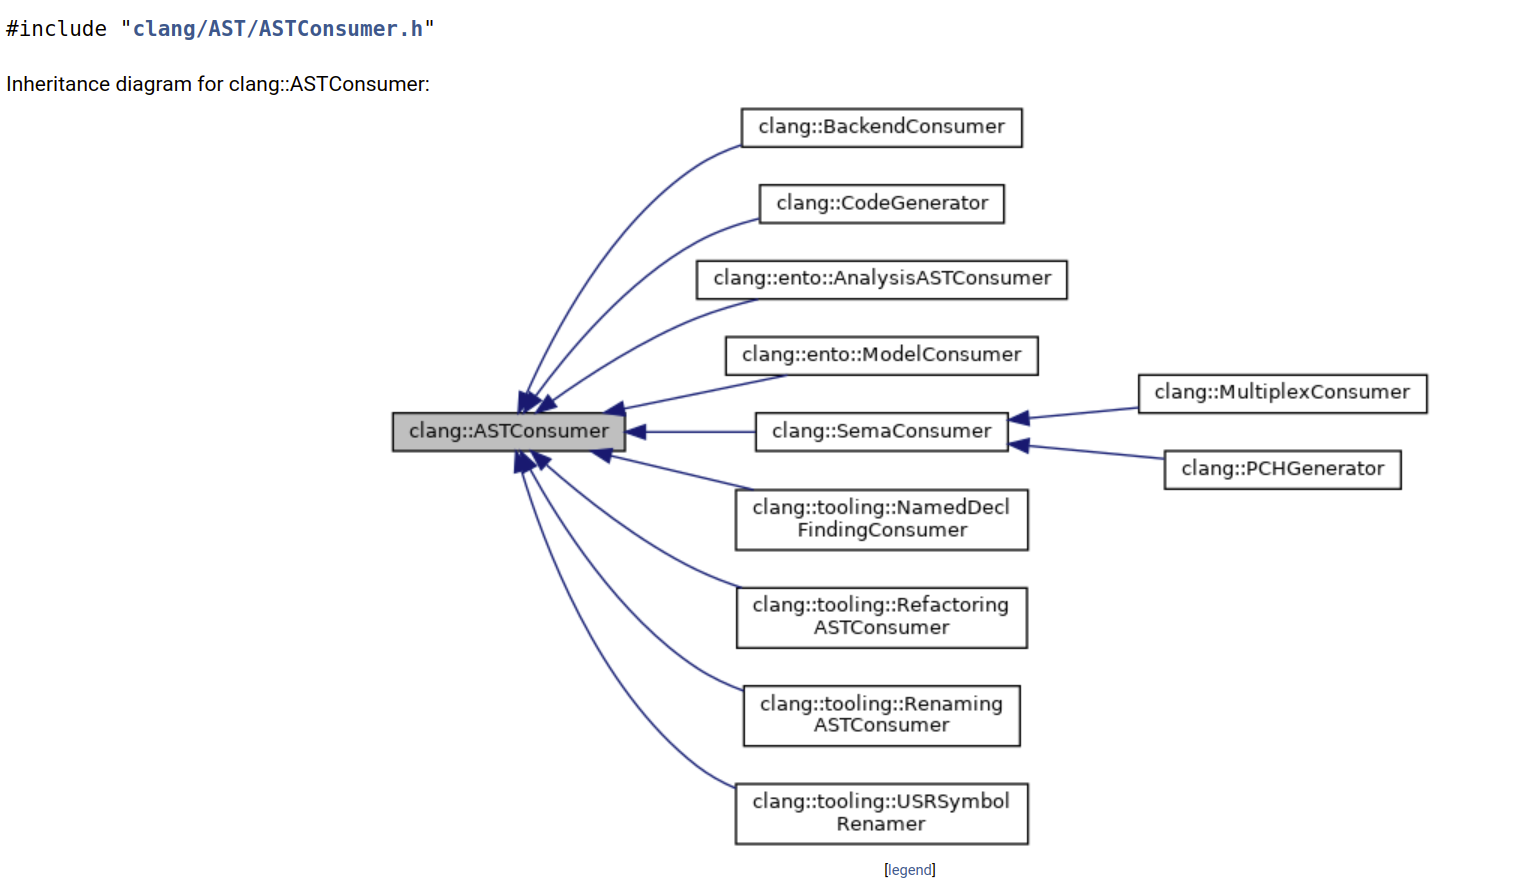
\includegraphics[scale=0.3]{ASTConsumer2.png}
\end{center}
\caption{Klase koje implementiraju \textit{\textbf{ASTConsumer}} interfejs}
\label{fig:exploded}
\end{figure}

Ovaj interfejs koristan je i za kreiranje samostalnih alata za stati\v{c}ku analizu koji se baziraju na analizi AST-a. U ovu svrhu mo\v{z}e se koristiti kombinacija
ovog interfejsa sa interfejsima za obilazak AST-a kao \v{s}to su AST posetioci i AST upariva\v{c}i. Klasa koja implementira neku analizu nad AST-om treba sadr\v{z}ati jedan ili vi\v{s}e objekata klasa za obilazak AST-a i zatim izvr\v{s}iti taj obilazak predefinisanjem metoda \textit{\textbf{virtual void  HandleTranslationUnit(ASTContext \&Ctx)}} koji se poziva nakon \v{s}to je kreiran AST za jedinicu prevodjenja. Logika same analize AST-a tokom obilaska treba biti implementirana u okviru klase koja implementira obilazak, odnosno u AST upariva\v{c}ima ili posetiocima.

\begin{lstlisting}[caption={Primer upotrebe klase \textit{\textbf{ASTConsumer}} u svrhu stati\v{c}ke analize}, label=simple]
class FindNamedClassVisitor
  : public RecursiveASTVisitor<FindNamedClassVisitor> {
public:
  bool VisitCXXRecordDecl(CXXRecordDecl *Declaration) {
    Declaration->dump();
    return true;
  }
};

class FindNamedClassConsumer : public clang::ASTConsumer {
public:
  virtual void HandleTranslationUnit(clang::ASTContext &Context) {
    Visitor.TraverseDecl(Context.getTranslationUnitDecl());
  }
private:
  FindNamedClassVisitor Visitor;
};
\end{lstlisting}

% UBACI SLIKU KODA KOMBINACIJE AST KONZUMERA I AST VIZITORA/MATCHERA






























% \end{itemize}


% ------------------------------------------------------------------------------

% \pangrami

% \pangrami

% ------------------------------------------------------------------------------
\chapter{Zaključak}
% ------------------------------------------------------------------------------
% \pangrami

% \pangrami

% ------------------------------------------------------------------------------
% Literatura
% ------------------------------------------------------------------------------
\literatura

% ==============================================================================
% Završni deo teze i prilozi
\backmatter
% ==============================================================================

% ------------------------------------------------------------------------------
% Biografija kandidata
\begin{biografija}
  % \textbf{Ognjen Plavšić} (\emph{Tršić,
  %   26. oktobar/6. novembar 1787. — Beč, 7. februar 1864.}) bio je
  % srpski filolog, reformator srpskog jezika, sakupljač narodnih
  % umotvorina i pisac prvog rečnika srpskog jezika.  Vuk je
  % najznačajnija ličnost srpske književnosti prve polovine XIX
  % veka. Stekao je i nekoliko počasnih mastera.  Učestvovao je u
  % Prvom srpskom ustanku kao pisar i činovnik u Negotinskoj krajini, a
  % nakon sloma ustanka preselio se u Beč, 1813. godine. Tu je upoznao
  % Jerneja Kopitara, cenzora slovenskih knjiga, na čiji je podsticaj
  % krenuo u prikupljanje srpskih narodnih pesama, reformu ćirilice i
  % borbu za uvođenje narodnog jezika u srpsku književnost. Vukovim
  % reformama u srpski jezik je uveden fonetski pravopis, a srpski jezik
  % je potisnuo slavenosrpski jezik koji je u to vreme bio jezik
  % obrazovanih ljudi. Tako se kao najvažnije godine Vukove reforme
  % ističu 1818., 1836., 1839., 1847. i 1852.
\end{biografija}
% ------------------------------------------------------------------------------

\end{document}
